\documentclass{article}
\usepackage[numbers,sort&compress]{natbib}
\usepackage{graphicx}
\usepackage{amsmath}
\usepackage{amssymb}
\usepackage{bm}
\usepackage{color}
\usepackage{tikz}
\begin{document}
\begin{abstract}
Classical Bretherton problem describes the propagation of gas fingers through liquid media with
thin liquid films between bubbles and the channel walls. The bubble shape and flow patterns are
complicated functions of the capilary number $Ca$ and Reynolds number $Re$. Recently we investigated
the applicability and parameters choice for the two-dimensional case Bretherton problem (flow
between plates) using the free-energy binary liquid lattice Boltzmann method (LBM)
\cite{kuzmin-binary2d}. This
work is the continuation of the previous work. It is focused on the three-dimensional capillaries
simulations with rectangular and square crosssections to
validate the binary liquid LBM for  Bretherton phenomena in the moderate range of the capillary
number $0.1\leq Ca \leq 1.0$.  
The flow is driven by a body force,
and
periodic boundary conditions are applied in the streamwise direction. The results show that the
binary liquid model is able to capture a number of phenomena happening in three-dimensional
capillaries, as the existence of the vortex in front of the bubble and the bubble radii dependency
on the capillary number. Therefore, the lattice Boltzmann free energy binary liquid model can be
used to simulate the Bretherton problem with good accuracy.
\end{abstract}

\section{Introduction}
The Taylor/Bretherton \cite{bretherton} flow deals with long gas bubbles moving through liquid in
narrow channels. Depending on the geometry it was found that the deposited film thickness
is a complicated function of the capillary number $Ca$:
\begin{equation}
\label{capillary:number:definition}
Ca=\frac{U_{\mathrm{bubble}} \mu_{\mathrm{liq}}}{\gamma},
\end{equation}
where $U_{\mathrm{bubble}}$ is the propagation bubble velocity, $\mu_{\mathrm{liq}}$ is the
kinematic liquid viscosity and $\gamma$ is the interfacial surface tension between gas and liquid. 

For example, the deposited film thickness
is proportional to $Ca^{2/3}$ in the range of small capillary numbers for circular channels
\cite{bretherton,heil-bretherton}. 
The problem of predicting flow patterns and associated mass transfers for the Bretheron-type flows
is of significant interests for chemical industry as it is widely used in chemical monolith
microreactors \cite{kreutzer-pressure-drop}. The large mass transfer can be achieved because of the
large interfacial area and small diffusion lengths \cite{cerro-bubble-train}. The heat transfer is
also increased in comparison with one phase flows \cite{fukugata-levelset}. While it
is possible to calculate the flow analytically for small capillary numbers \cite{bretherton}, it's
not possible to extrapolate it to the wider range of capillary and Reynolds numbers used in the
chemical
industry. Thus, the desire of consistent numerical simulations arises.

The two-dimensional geometry (circular tubes, parallel plates) flows are studied extensively in
experimental works of \citet{aussillous-deposition, cerro-bubble-train} and numerical works of
\citet{giavedoni-numerical,heil-bretherton}. All abovementioned works found that the Bretherton
analysis is valid only for small capillaries numbers $Ca\leq 0.003$ and deviates for larger ones.
That is caused by complex interplay of the gravitational,
interfacial, inertial and viscous forces \cite{gupta-review}. Historically, 
\citet{bretherton} indicated that inertia effects can be 
neglected. \citet{giavedoni-numerical} suggested
that
inertia effects
are negligible for $Ca \leq 0.05$ and have moderate changes for $Ca>0.05$ in the range of Reynolds
number from $0$ to $70$ for two-dimensional geometry flows. Later on, \citet{heil-bretherton}
extended
results for the flow between plates upto Reynolds number
$300$. They indicate that while the influence of the established film thickness is insignificant
($7$ percent from the film thickness measured at $Re=0$), the change in Reynolds number 
influences significantly the pressure distrubution and the flow field near the front bubble tip.
\citet{cerro-bubble-train} show that the mass transfer is strongly affected by flow direction for
small capillary numbers in case of upward and downward flows. Thus, to fully describe the
propagation of the semi-infinite finger in liquid media one needs to take into the account the
viscous, gravitational, surface and inertia forces \cite{gupta-review}.  

In comparison with the two-dimensional Bretherton flow  (circular tubes, flow between
parallel
plates), there is a vast number of experimental
results available for the three-dimensional case as microchannels with square, triangular and
rectangular crosssections. For instance, \citet{cerro-bubble-train} performed a number of
experiments for a
bubble-train flow in capillaries of
circular and square cross section for horizontal, upward and downward flows.
\citet{shikazono-square} obtained
experimental
results for the deposition length dependency on the
capillary number for ethanol/air and water/air mixtures and for square, circular and triangular
shaped mirochannels. They also found experimental correlation for the prediction of bubble radii
based on the capillary number $Ca$ and the Weber number $We=Re\,Ca$. 

In comparison with two-dimensional geometries, the experimental works
\cite{shikazono-square,cerro-bubble-train} supported by numerical simulations \cite{heil-threedim,
wang-non-circular} show interesting phenomena in three-dimensional geometries. It was found
\cite{heil-threedim,wong-films} that for rectangular
or square shaped capillaries there is a transition for a
certain capillary number, where the bubble crosssection changes from the non axisymmetric to axis
symmetric case. Non axisymmetric case is attributed to the case where the axial radius is
different from the
diagonal radius and the bubble has the non-circular shape in the channel crossection. In this case
the bubble shape mimics the shape of the square and looks like a rounded square. The dependence
of the diagonal and axial radii on the capillary number is shown in Fig. 
\ref{fig:heil:three:dim}.
\begin{figure}[ht]
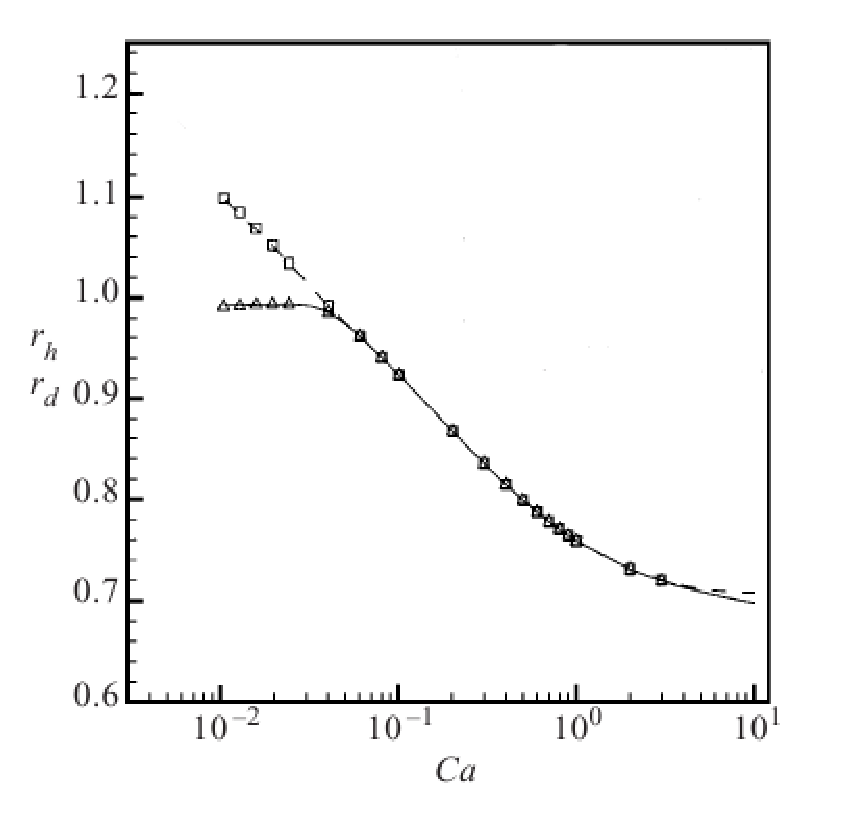
\includegraphics[width=\textwidth]{Figures/capillary_width_heil.eps}
\caption{\citet{heil-threedim} results for the variation of the deposited liquid for the range of
capillary number. One can see the asymmetry between diagonal and axis diameter for the capillary
number $Ca\leq\hat{Ca}=0.04$. Courtesy of \citet{heil-threedim}. \label{fig:heil:three:dim}}
\end{figure}
The transition number between non-axisymmetric case and symmetric is indicated in a number of
works as $\widehat{Ca}=0.04$ \cite{cerro-bubble-train},
$\widehat{Ca}=0.1$
\cite{cerro-space,wang-non-circular}, $\widehat{Ca}=0.033$ \cite{heil-threedim}. If the capillary
number is larger
than
the critical capillary number, i.e. $Ca>\widehat{Ca}$, then the bubble becomes axisymmetric with the
radius of the droplet dependant on the capillary number. One of the example for the bubble radii
dependence on the capillary number is in Fig. \ref{fig:heil:three:dim}.

There are also a number of numerical works for the three-dimensional case. For instance, 
\citet{wong-films,wong-pressure} studied
three-dimensional bubbles in
polygonal capillaries and calculated bubble shapes for different
slug and bubble cross sections and menisci appearance.
\citet{heil-threedim} performed three-dimensional simulations for circular shaped,
square and rectangular shaped capillaries. They indicated the transition
capillary number where the streamlines pattern
changes from having a vortex in front of the bubble and not having it for larger capilllary
numbers, {\color{red} Fig. \ref{fig:streamlines:pattern} }. For the square channel the critical
capillary number is $Ca=0.691$.  Authors also found an empirical correlation which
allows to put
different aspect ratio rectangular channels simulation results on one
curve. It is also indicated that for certain aspect ratio microchannels $\alpha=\frac{a}{b}\geq
2.04$ the interface can not make up the
axisymmetric case for any capillary number. \citet{wang-non-circular} performed numerical
simulations by the VOF technique for the
non-circular
shaped capillaries as square and triangular shaped capillaries. They also investigated the relative
velocity of the bubble for
different capillary numbers. 

As it is mentioned by \citet{gupta-review}, the most common techniques to simulate the Bretherton
phenomena are the Volume of Fluid (VOF) method \cite{wang-non-circular}, the level-set method
\cite{fukugata-levelset} and the finite element methods \cite{kreutzer-taylor,heil-threedim}. It is
also indicated \cite{gupta-review}, that the new techniques which are still in the development stage
are the lattice Boltzmann method and phase field methods \cite{anderson-diffuse,gurtin-binary}.
While the finite element methods solve the Bretherton flow as a free-surface problem with a sharp
interface but without underlying details for gas, the lattice Boltzmann method which is a continuous
interface method arises as a promising alternative for simulation of gas finger propagation. The
continuous interface has more flexebility in simulations involving coalescence and/or droplet
breakup.

In our previous work \cite{kuzmin-binary2d} we already covered the Bretherton flow between plates.
It was shown that the free-energy binary liquid model, which is a phase field method, simulates
with reasonable accuracy the Bretherton/Taylor phenomenon. The goal of this work is to examine the
three-dimensional geometry simulations conducted by the free-energy binary liquid lattice Boltzmann
method. We focus on the feasibility study of the numerical method for the microchannels with
square crosssections. 


The lattice Boltzmann method has emerged as a successful method to simulate
a wide variety of phenomena including hydrodynamics \cite{yu}, thermal flows
\cite{karlin-minimalmodels}, microflows \cite{ansumali-small-knudsen},
ferrofluids \cite{kuzmin-aniso}, and multiphase flows
\cite{swift,Shan-chen:extended}. The method is a particle method which allows to simulate physical
phenomena on the microscopic level. For instance, the introduction of the force or potential on the
microscopic level allows to restore multiphase macroscopic equations \cite{swift,
Shan-chen:extended}.

The binary liquid free-energy LB model due to \citet{swift} we used
simulates two liquids with the assumption of uniform overall
density. While the classical Bretherton problem is stated for gas and liquid, which are of
significantly
different densities and viscosities, the parameters were carefully chosen as to neglect the inertia
effects, see Section \ref{sec:numerical:benchmark}. Moreover, the results of
\citet{giavedoni-numerical} and \citet{heil-bretherton} show
negligible Reynolds number effects on the film thickness for a relatively wide range of Reynolds
numbers. Thus, a major governing factor for microchannel flows is not the density ratio, but
the
viscosity ratio. That is why the uniform density binary liquid model is suitable for this kind of
simulations. The goal of this work is to do a feasibility study of the LBM
binary-liquid model to simulate and correctly predict flow patterns for the Bretherton/Taylor
problem. The work results are in good agreement with other simulations
\cite{heil-threedim,wang-non-circular}. 

One should also acknowledge the works of \citet{pagonabarraga-fingers} on menisci
in thin films for fingering phenomena. \citet{sehgal-microchannel} performed lattice Boltzmann
simulations of two-dimensional channel flows for relatively large capillary numbers, and
found discrepancies with the classical Bretherton theory, which
is limited to the low capillary number regime \cite{giavedoni-numerical}. The Shan-Chen model was
used to simulate the Bretherton problem, which is sometimes referred to contain thermodynamically
inconsistent interface \cite{nourgaliev-breakup}. 

The paper is organized as follows.  First, we explain the simulation benchmark construction
mainly based on our previous work \cite{kuzmin-binary2d}. Then, the binary liquid lattice
Boltzmann model is outlined. The simulation results for the three-dimensional case are presented in
the results section. The results cover the film thickness dependency on the capillary number, the
relative velocity of the bubble and the vortex profiles. The paper
is concluded with a summary of the main findings.
%The critical capillary numbers for changing velocity pattern depending on the eccentricity
%parameter $\alpha$ are presented in Table \ref{table:recirculation:data}.
%\begin{table}
%\begin{tabular}{c|c}
%$\alpha$& $Ca_{T}$\\
%\hline
%1& 0.691\\
%1.1 & 0.688\\
%1.3 & 0.666\\
%1.5 & 0.631\\
%\end{tabular}
%\caption{The results for the recirculation region.\label{table:recirculation:data}}
%\end{table}

\section{Numerical benchmark approach}
\label{sec:numerical:benchmark}
The main discussion here follows and is based on the two-dimensional benchmark approach
\cite{kuzmin-binary2d}. It was indicated that the benchmark layout should have certain
dimensions to conduct simulations. The classical Bretherton benchmark layout is represented in Fig.
\ref{fig:classical:benchmark}. It describes the gas finger propagation through the liquid media.
The film thickness in this case is measured at the inlet. In lattice Boltzmann framework such
formulation has certain challenges \cite{kuzmin-binary2d}. Some of them are attributed to the
dynamic coupling of the inlet and outlet conditions \cite{giavedoni-numerical}. Instead, we
proposed the numerical benchmark indicated in Fig. \ref{fig:lbm:benchmark}. The dimensions of the
channel are chosen as $H_{\mathrm{eff}}\times H_{\mathrm{eff}} \times 15 H_{\mathrm{eff}}$. The
initialized bubble length is taken as $5 H_{\mathrm{eff}}$.\citet{giavedoni-numerical} showed that
the film stabilizes at the distances of $2.6-4.0$ diameters
from the front tip depending on the Reynolds number.  We chose to measure the film thickness in the
middle of the bubble, which is located at least at a distance of $2.5-3$ channel heights from the 
bubble tip. Moreover, the film thickness examination, see Section
\ref{section:film:thickness:variation}, shows that for the capillary range of interest, i.e.
$0.05\leq Ca \leq 1$, the standard deviation of the film thickness from the bubble middle film
thickness is around $7$
percent for small capillary numbers ($Ca=0.05$) and less than $1$ percent for larger ones ($Ca
\geq 0.1$). %at the distances one channel height from the rear tip upto one channel


This length of the bubble was shown as
sufficient for the film thickness to stabilize.   

\begin{figure}[ht]
\includegraphics*[bb=153 610 405 717,width=\textwidth]{Figures/benchmark_classical.eps} 
\caption{The classical benchmark. The semiinfinite gas bubble
propagates through the liquid media. \label{fig:classical:benchmark}}
\end{figure}[ht]
\begin{figure}
\includegraphics*[bb=152 480 410 713,width=\textwidth]{Figures/benchmark_lbm.eps}
\caption{The classical benchmark. The semiinfinite gas bubble
propagates through the liquid media. \label{fig:lbm:benchmark}}
\end{figure}



 In order to avoid the mutual 


It was indicated that the film thickness should be at least as twice large
as the interface thickness. The interface thickness in the continuous formulation of the
free-energy binary liquid formulation occupies $3-5$ nodes. Therefore, the film should be
resolved at least as $6-10$ nodes. 

As it was indicated before \cite{heil-threedim}, the diagonal bubble radius is different from the
axial bubble radius for $Ca\leq \widehat{Ca}\approx 0.05$. The radii coincide for larger values of
$Ca$, but the value of bubble radii is $R_{diag}=R_{axis}=0.99 a$, where $a$ is the side length of
the square microchannel. Therefore, taking the minimal requirement for the film thickness to be
resolved, i.e. $6$ lattice nodes, one can obtain the grid size as $600\times 600 \times $ to
simulate 

Non axisymmetric case is attributed to the case where the axial radius is different from the
diagonal radius and the bubble has the non-circular shape in the channel crossection. 
{\color{red}
\citet{cerro-space} indicate that because of asymmetry the flow in the corner can predominate the
flow in the side of the capillary thus changing the qualitative differencies depending on the
gravity direction. ``Because of the mixing, the gas-liquid mass tranfer coefficient are 2-5 times
larger fro upflow than for downflow''. 
}

Most multiphase lattice Boltzmann models \cite{swift, Shan-chen:extended} resolve
the interface using continuous interface methods where the interface spans over several grid nodes.
Such a representation
brings issues of the film thickness resolution versus interface
resolution -- the diffuse interface should be dealt with in such a way as to have a
negligible effect on the physics of the film. In our previous work \citet{kuzmin-binary2d} the grid
resolution was examined. It was found that the film thickness should be at least as twice as the
interface for the simulation to be accurate.



Therefore, the major governing parameter for microchannel Bretherton flows is not the density ratio,
but the
viscosity ratio. Thus, the applicability of the binary liquid model can be examined for the
simulation of the square shaped capillaries.

 Moreover, the results based on uniform density, as in the case of the LBM
binary liquid model, are in good agreement with other simulations
\cite{giavedoni-numerical,heil-bretherton} in which inertia effects were taken into account. The
same indicated in \cite{gupta-review} the  classical Bretherton problem is stated for
gas and liquid, which are of
significantly
different densities and viscosities.


Resolving the interface on a fine level for capillary numbers smaller than
$0.003$ is computationally expensive even in the two-dimensional case
(the amount of memory necessary to perform the simulation would be of the order
of tens or hundreds of gigabytes).  This work is therefore based on a
comparison of the results obtained with the known data
validated for the Bretherton bubble flow.  In this paper, we present
techniques for initialization of the simulations and discuss optimal
parameter ranges for the binary liquid LB model, such as the binary liquid parameters, the viscosity
ratio and the grid resolution. The emphasis is to obtain correct flow physics, especially in terms
of film thicknesses.





The VOF technique is the continuous
interface method based on a non-uniform grid. It is of particular interest for us to compare it
with the continuous interface method by the LBM implementation. 



Thus, there is the effect of
inertia on the bubble formation. 


Recent experimental results by \citet{shikazono-square} for square shaped capillaries indicate the
following dependency on the capillary number $Ca$ and the Weber number $We$:
\begin{equation}
\begin{aligned}
&R_{diag}=1.171-\frac{2.43 Ca^{2/3}}{1+7.28 Ca^{2/3}-0.255 We^{0.215}}\\
&R_{axis}=
\begin{cases}
1, &R_{diag}>1\\
R_{diag}, &R_{diag}\leq 1.
\end{cases}
\end{aligned}
\end{equation}
In the present
simulations the largest Reynolds number we achieve is less than $1$ and the capillary number is of
order of unity. Thus, it allows to neglect 
inertia effects. 




\section{Steady-state case}
We performed different simulations to understand a number of steps required for the problem to come
on the steady-state. The grid to be simulated is $52\mathrm{x}52\mathrm{x}750$ which simulates the
quarter of the channel with the initial
width as $6.5$ lattice Boltzmann units together with $\frac{\mathrm{d}P}{\mathrm{d}x}=1.6
\mathrm{x}10^{-6}$. The simulation was performed for $140000$,$150000$,$160000$, $170000$ and
$180000$ iterations. The results are summarised in Table \ref{table:steady:state}. Whole the
capillary number varies only in the 4th digit, radiuses are one percent accurate. 

As well we performed longer simulations in the range of moderate capillary numbers after
$140000$, $160000$, $180000$, $200000$, $220000$, $240000$. The results for the capillary number
based on the bubble velocity in the middle crossection are shown in Table \ref{table:steady:state}. 
%{\color{red} What is it One of the
%profiles in
%the middle of the bubble is shown in Fig. \ref{fig:steady:state:profile:example}. }
\begin{table}
\begin{center}
\begin{tabular}{|c|c|c|c|}
\hline
$N_{iter}$&$Ca$&$R_{axis}$&$R_{diag}$\\
$140000$&$0.0532$&$0.9379$&$1.075$\\
$150000$&$0.0533$&$0.9375$&$1.072$\\
$160000$&$0.0535$&$0.9372$&$1.069$\\
$170000$&$0.0536$&$0.9369$&$1.066$\\
$180000$&$0.0537$&$0.9366$&$1.062$\\
\hline
\end{tabular}\\
\begin{tabular}{|c|c|c|c|}
\hline
$N_{iter}$&$Ca$&$R_{axis}$&$R_{diag}$\\
$140000$&$0.3578$&$0.8657$&$0.8708$\\
$160000$&$0.3590$&$0.8650$&$0.8702$\\
$180000$&$0.3598$&$0.8647$&$0.8700$\\
$200000$&$0.3603$&$0.8645$&$0.8698$\\
$220000$&$0.3607$&$0.8644$&$0.8697$\\
$240000$&$0.3609$&$0.8645$&$ 0.8697$\\
\hline
\end{tabular}
\end{center}
\caption{Underresolved capillary number results and resolved Results for the steady-state case. One
can see that $200000$ steps are enough to structure
the bubble. \label{table:steady:state}}
\end{table}

%\begin{figure}
%\includegraphics[width=0.47\textwidth]{Figures/bullet.eps}\hfill
%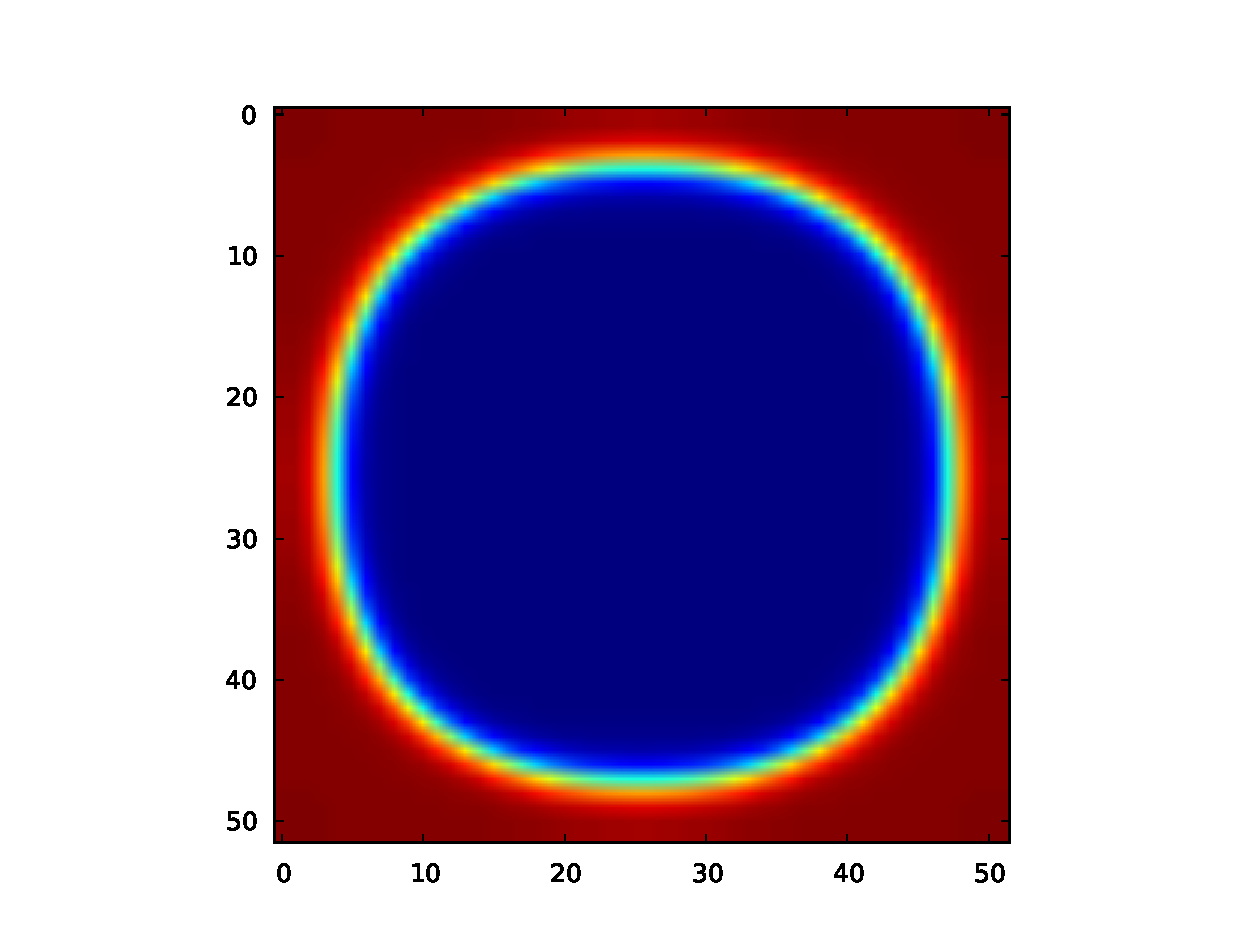
\includegraphics[width=0.47\textwidth]{Figures/example_crossection.eps}\\
%\caption{Slice in the middle of the bubble and
%three-dimensional example. \label{fig:steady:state:profile:example}}
%\end{figure}

\section{Non-axisymmetric case}
We first start with the non-axisymmetric case. As it was indicated before for a quite low capillary
number the flow becomes axisymmetric. For
example, according to \cite{heil-threedim} for the capillary
number $Ca=0.01$, the axis and diagonal radiuses are $r_h=0.99$ and $r_d=1.1$ respectively.
Therefore the film thickness in the axial direction is  $0.5\%$ of whole channel width to see the
difference. Our previous calculations \cite{kuzmin-binary2d} show that the film thickness should be
 resolved around $40-50$ percent for calculations to be convergent and grid independent. This
condition certainly implies a large grid with the computational high demand. For instance, to
properly simulate the abovementioned example the grid should be as 
$200x200x3000$ nodes. In this section we want to examine the assumption of the underresolved
interface whether it can produce the consistent film thicknesses for low capillary numbers. The
interface occupies around $1-2$ lattice units. 

Here we present simulations for the domain of size $52\mathrm{x}52\mathrm{x}1500$ which simulates
the quarter of the channel using the mirror boundary conditions (See Appendix \ref{append:sym}).
That
results in the effective grid size as $100\mathrm{x}100\mathrm{x}1500$. The simulation is carried
out with the pressure gradient as:
\begin{equation}
\frac{\mathrm{d}P}{\mathrm{d}x}=1.6\,10^{-6}.
\end{equation}
The initial film thickness was taken as $6$ nodes. 

One can see the phase profile in the middle of the bubble in
Fig.\ref{fig:quarter:capillary:capillary01}. For comparison reason the axisymmetric phase profile
for $Ca=0.6$ is presented in Fig. \ref{fig:bubble:axisymmetric}. The associated capillary number is
$0.053$ based on
the calculation of the bubble velocity in the center of the bubble. The radiuses in this simulation
are as $R_{axis}=0.93$ and $R_{diag}=1.06$. While $R_{axis}=0.93$ is underestimated parameter and
we can't take into the consideration apriori, one can consider parameter $R_{diag}=1.06$ the
parameters for the capillary number $0.053$ should be according to \citet{heil-threedim} as $0.97$
and $1.05$ according to the VOF simulations of \citet{wang-non-circular}. One can conclude that
even though the axis film thickness is not properly resolved the diagonal values are consistent and
can give an approximate information. 
\begin{figure}
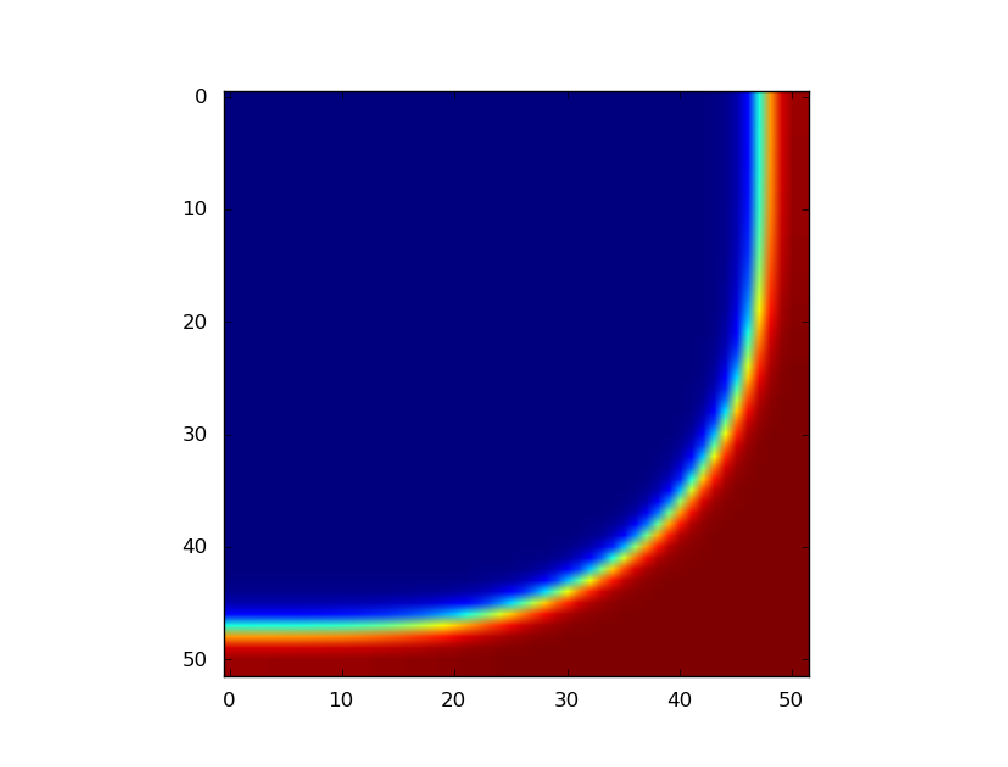
\includegraphics[width=0.97\textwidth]{Figures/quarter.eps}\\ %\hfill
\includegraphics[width=0.97\textwidth]{Figures/stream_cap01.eps}\\
\caption{Streamlines and phase profile of the quarter of the channel. The capillary number is
$0.053$ and the film thickness is underresolved. \label{fig:quarter:capillary:capillary01}}
\end{figure}
\begin{figure}[ht]
\includegraphics[width=0.97\textwidth]{Figures/square.eps}
\caption{The middle bubble phase profile. One can see that the diagonal radius coincides with the
axial radius. {\color{red} $Ca=0.5$} \label{fig:bubble:axisymmetric}}
\end{figure}


For underresolved schemes we performed a number of simulations on a GPU code with the grid of size
$50\mathrm{x}50\mathrm{750}$. While changing the applied force in a manner indicated in Appendix
\ref{append:scaling} the velocity of the bubble was increased to obtain larger capillary numbers,
see Fig. \ref{fig:underresolved:capillaries}. One can see that the deviation between the diagonal
and axial radiuses are quite significant and they coincide only when the interface is resolved
($Ca\approx 1.0$). In calculations with better grids, i.e. quarter channels simulations on CPU, the
axial radius coincides with the diagonal in the $0.5\%$ range. Moreover, the capillary number curve
resembles already published date of \citet{heil-threedim} in a better way, see Fig.
\ref{fig:capillary:comparison}. 
\begin{figure}[ht]
\includegraphics[width=0.97\textwidth]{Figures/underresolved_capillaries.eps}
\caption{The underresolved profiles axis and diagonal radiuses versus capillary numbers. $50$
percent resolution starts from $Ca=1.0$, which is quite high. One can see it's exactly where
radiuses converge instead of $Ca=0.04$. {\color{red} To delete? However, one can see from
simulations Fig.
\ref{fig:wang:critical:capillary} and Fig.\ref{fig:thickness:variation:ca:ten} the thickness,
especially for Fig.\ref{fig:thickness:variation:ca:ten}, can significantly variate over a bubble
length.} \label{fig:underresolved:capillaries}}
\end{figure}

\section{Velocity pattern}
We examined two different velocity patterns to identify change of pattern. Two capillaries numbers
were taken below and above the numbers indicated in Table \ref{table:recirculation:data}, as
$Ca=0.36$ and $Ca=0.88$.Velocity streamlines are
indicated in Fig. \ref{fig:streamlines:pattern}. One can see that the vortex indicated in
Fig.\ref{fig:heil:recirculating} doesn't appear in present calculations. This fact can be
explained because the simulation is carried our for the binary-liquid case but not free-surface
interface presented in the classical Bretherton problem. In the latter case the void phase pushes
the liquid towards the walls. In the present simulation there is no a void phase. Then the
streamlines have the ability to go through the interface and we exactly see this situation occuring.
\begin{figure}[ht]
\includegraphics[width=0.97\textwidth]{Figures/streamlines_ca036.eps}\\
\includegraphics[width=0.97\textwidth]{Figures/streamlines_ca088.eps}
\caption{Streamlines for $Ca=0.36$ and $Ca=0.88$. One can see that there are no vortexes created
before the bubble. It can be explained by the fact that the binary-liquid model is simulated
instead of free-surface interface gas air finger flow.\label{fig:streamlines:pattern}}
\end{figure}

\section{Variation bubble length}
The works of \citet{heil-threedim} of \citet{wang-non-circular} show the variation of the bubble
thickness through the length of
bubble. The length variation is presented in Fig.\ref{fig:thickness:variation:ca:ten} and
Fig.\ref{fig:wang:bubble:shape}. While Fig. \ref{fig:wang:bubble:shape} indicates that the diagonal
radius has a variation for the rather small capillary numbers as $Ca<0.1$, another profile is
presented for the $Ca=10$ and shows the variation for the diagonal radius. We examined a bunch of
different capillaries numbers to present the diagonal radius variations over the length:
The axis and diagonal radiuses variation over the bubble are shown in Figure
\ref{fig:bubble:variation:capillaries}. The rather small capillary numbers one can see the increase
in the rear menisci of the diagonal radius which coincides with the results of
\citet{wang-non-circular}. One can see that variation over the length can be neglected
for relatively high $Ca$ numbers. 
\begin{figure}[ht]
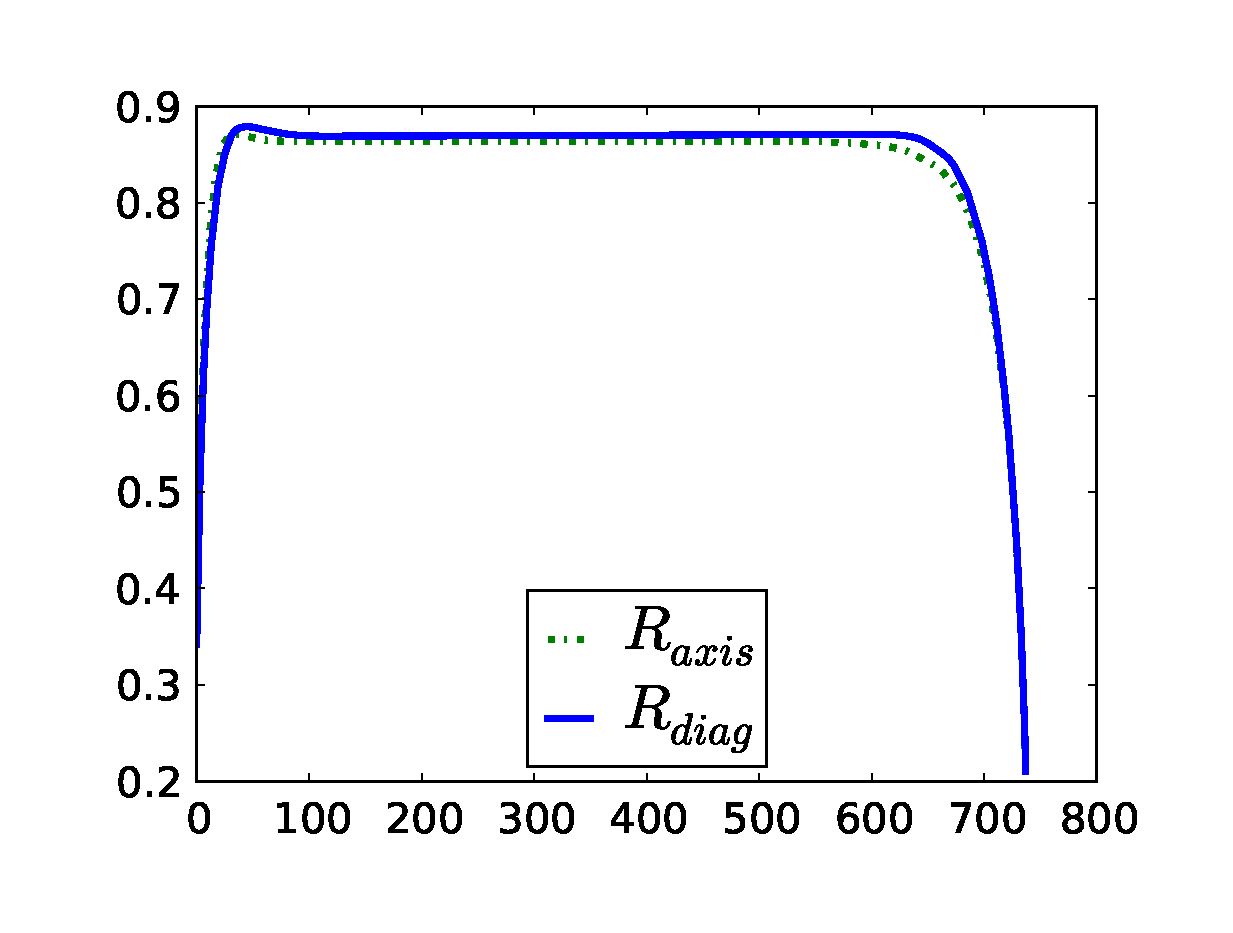
\includegraphics[width=0.47\textwidth]{Figures/bubble_length_ca_36.eps}\hfill
\includegraphics[width=0.47\textwidth]{Figures/bubble_length_ca_46.eps}\\
\includegraphics[width=0.47\textwidth]{Figures/bubble_length_ca_61.eps}\hfill
\includegraphics[width=0.47\textwidth]{Figures/bubble_length_ca_88.eps}\\
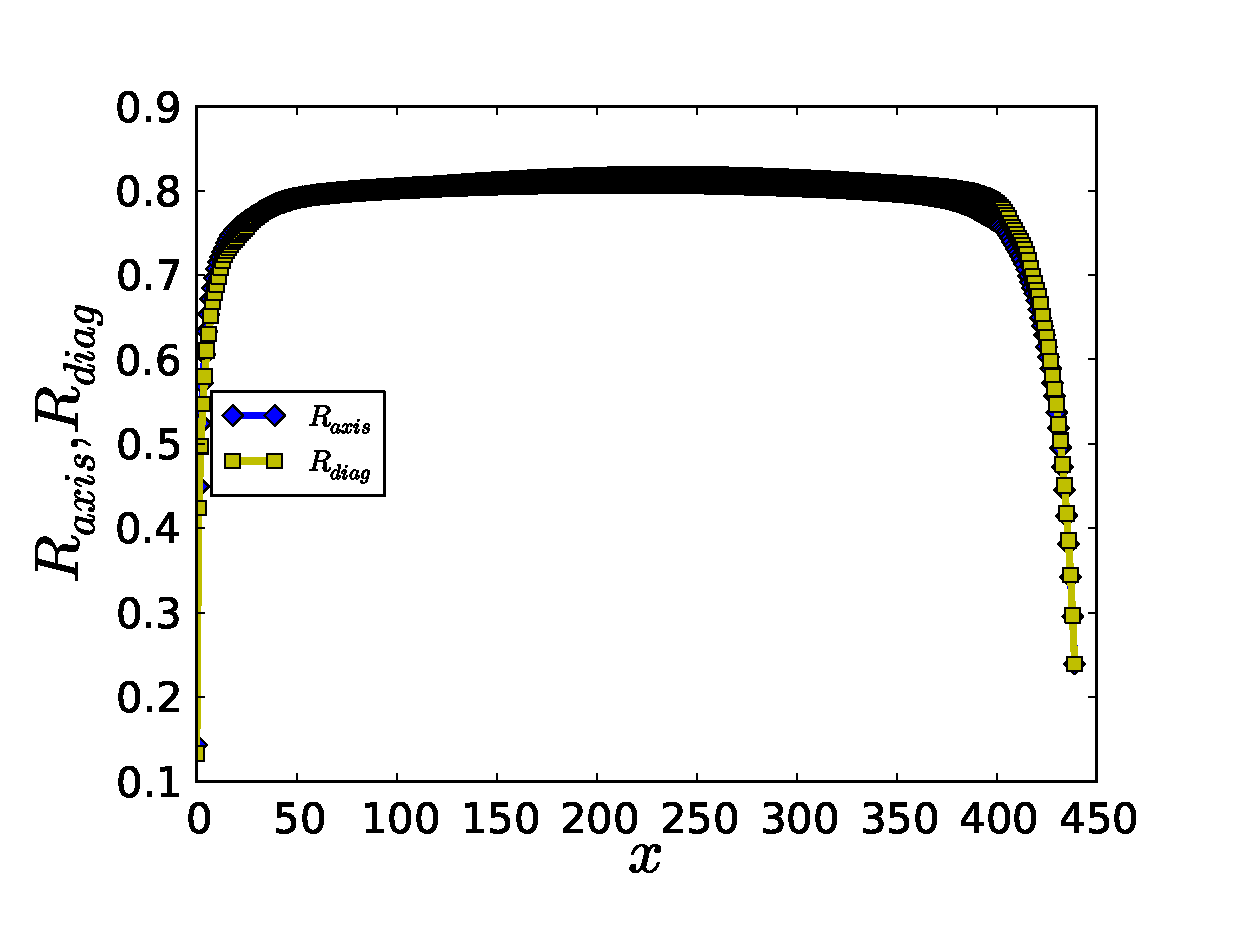
\includegraphics[width=0.47\textwidth]{Figures/bubble_length_ca_one.eps}
\includegraphics[width=0.47\textwidth]{Figures/bubble_length_ca_117.eps}
\caption{The radiuses variations for the capillary number $Ca=0.46$.
One can see the diagonal radius different from the axial radius near the front of the tip which is
somehow coincides with the results of
\citet{heil-threedim}. The results are presented for the
capillary numbers (from left to right, top to bottom)
$0.36$,$0.46$, $0.61$, $0.88$,$1.06$,$1.17$. \label{fig:bubble:variation:capillaries}}
\end{figure}
\begin{figure}
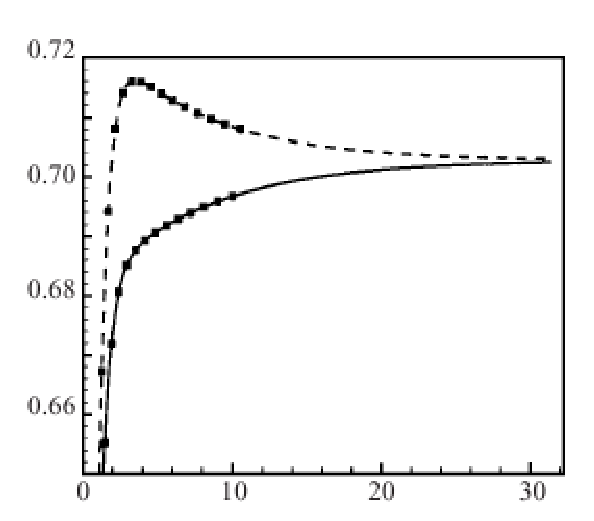
\includegraphics[width=0.97\textwidth]{Figures/variationoverlength.eps}
\caption{The variation of the bubble length for capillary number $Ca=10$. The x-axis scaled to
half-width of the microchannel height.  \label{fig:thickness:variation:ca:ten}}
\end{figure}

Concerning results indicated in Fig.
\ref{fig:thickness:variation:ca:ten} simulations are unstable that means one needs to work with
small surface tension ({\color{red} See results of Pagonabarraga}). One can see that the difference
between diagonal radius and
usual radius is of order of $4\%$. That means it's 2 percent of the channel height. If the
simulation is conducted by the grid $100\mathrm{x}100$ in the cross section that means that we will
see the difference in two grid nodes. Therefore the grid is $102\mathrm{x}102\mathrm{1500}$. It is
known from simulations that for the grid $102\mathrm{x}102\mathrm{x}1500$ the largest force gradient
is $2\mathrm{x}10^{-5}$ with free energy binary liquid parameters $A=0.04$,$k=0.04$ and $Ca\approx
1.0$. Therefore, we want to keep the same body force but to obtain larger capillary number. That
can be done through the scaling indicated in Appendix \ref{append:scaling}:
\begin{equation}
\frac{\mathrm{d}P}{\mathrm{d}x}\propto \gamma Ca .
\end{equation}
Therefore the same body force can stand for capillary number ten times larger if the surface
tension is ten times smaller:
\begin{equation}
\gamma=\sqrt{\frac{8 k A}{9}}.
\end{equation}
The following can be satisfied if $A=0.004$ and $k=0.004$. Decreasing surface tension requires
increasing the mobility of the interface to be able to adjust to the interface
\cite{pagonabarraga-parameters}. We therefore performed the numerical simulation with those
parameters and $\Gamma=20$ for the interface to be stable. 
{\color{red} However, many authors state that increasing mobility kills
the
proper results of simulations}.
{\color{red} Need to wait results from bugaboo.westgrid.ca under LargeCap simulation}

\section{Capillary number}
We performed a number of simulations with quarter CPU code and GPU train simulations and compared
them with data obtained by \cite{heil-threedim}. After performing the simulations we determine the
$R_{axis}$, $R_{diag}$ versus calculated
capillary number
\begin{equation}
Ca=\frac{\mu_{liq} U_{bubble}}{\gamma}.
\end{equation}
To perform simulations we
started with the following parameters as
$k=0.04$,$A=0.04$,$\Gamma=1.0$. We performed different grids calculations with GPU and CPU codes.
The GPU code (see section \ref{section:bubble:train} about bubble train simulations) simulates a
quarter of the bubble and operates on the grid $100\mathrm{x}100\mathrm{x}1500$. The CPU refined
grid operates on whole $160\mathrm{x}160\mathrm{x}1500$. In this case we see short bubbles as the
length to height ratio is $\frac{500}{160}=3.125$. GPU  For GPU grids due to memory constrains we
chose the grid as $N_x\mathrm{x}N_y\mathrm{x}N_z=52\mathrm{x}52\mathrm{x}750$. One can see the
comparison presented in Fig. \ref{fig:capillary:comparison}.
\begin{figure}
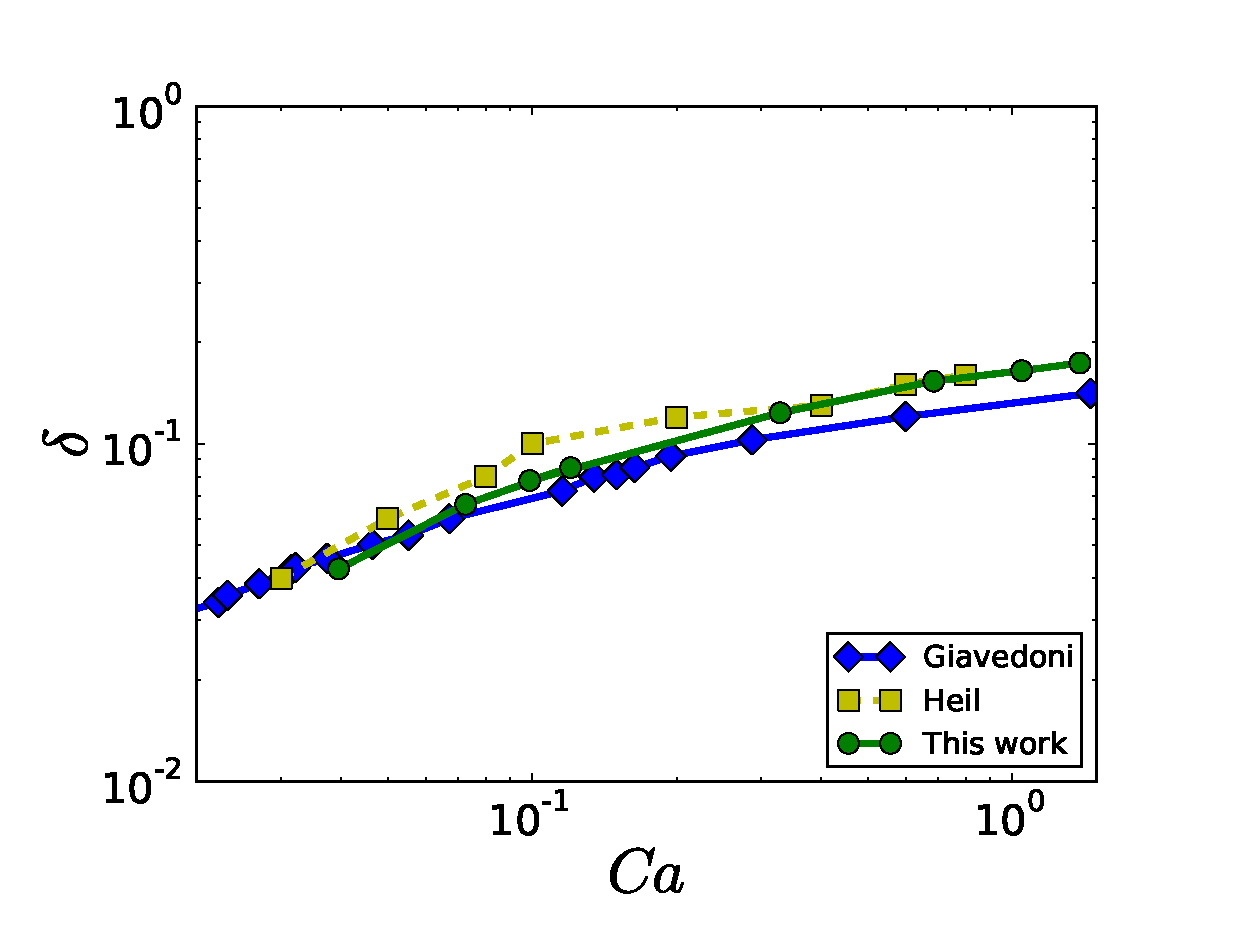
\includegraphics[width=0.97\textwidth]{Figures/capillaries_comparison.eps}
\caption{The comparison between different runs of codes for the axial and the diagonal radiuses
versus capillary numbers. \label{fig:capillary:comparison}}. One can see that the code mimics
behavior of the earlier published results.
\end{figure}


\section{Train simulation}
\label{section:bubble:train}
As far as the requirements for the grid are ``heavy'' we performed a bunch of simulations to
examine how the distance between bubbles influences on the thickness. For this purpose the
simulation was conducted on the grid 82x82x750. We examined different initialized distances between
bubbles. The initial lengths of bubbles were chosen as $300$, $350$, $400$, $450$, $500$, $550$
lattice units. Therefore, the corresponding initial distances between bubbles are
$450$,$400$,$350$,$300$,$250$ lattice units. On the steady state regime the distances become $386$,
$317$, $248$,$176$,$99$,$23$ lattice units. The corresponding capillary numbers calculated based on
the center bubble velocity are as follows $0.905$, $0.986$,$1.08$,$1.19$, $1.33$, $1.49$. The
calculated radiuses (diagonal radius equal to the axes radius) are as follows
$0.783$,$0.778$,$0.772$,$0.764$,$0.753$,$0.747$. Thus, one can see the great impact of the bubbles
on each other velocity for the given body force. However, in terms of the film thicknesses those
numbers look adequate. One can see the film thicknesses dependency on the capillary number for
simulations obtained by \citet{heil-threedim} and bubble train simulations data in Fig.
\ref{fig:capillaries:train} and in Fig. \ref{fig:capillary:comparison}. One can see that the
results are consistent and in a good agreement.
Therefore, though the bubble train mutual motion influences on the film thickness by increasing the
associated capillary number,  however, the film thickness is in accordance with the capillary
number correlation. Thus, the decrease of the numerical domain is quantified and can be used to
obtain the data. However, one should be cautious about the initialization, because the Poiseuille
flow initialization is deviated even further due to mutual motion of bubbles.
\begin{figure}
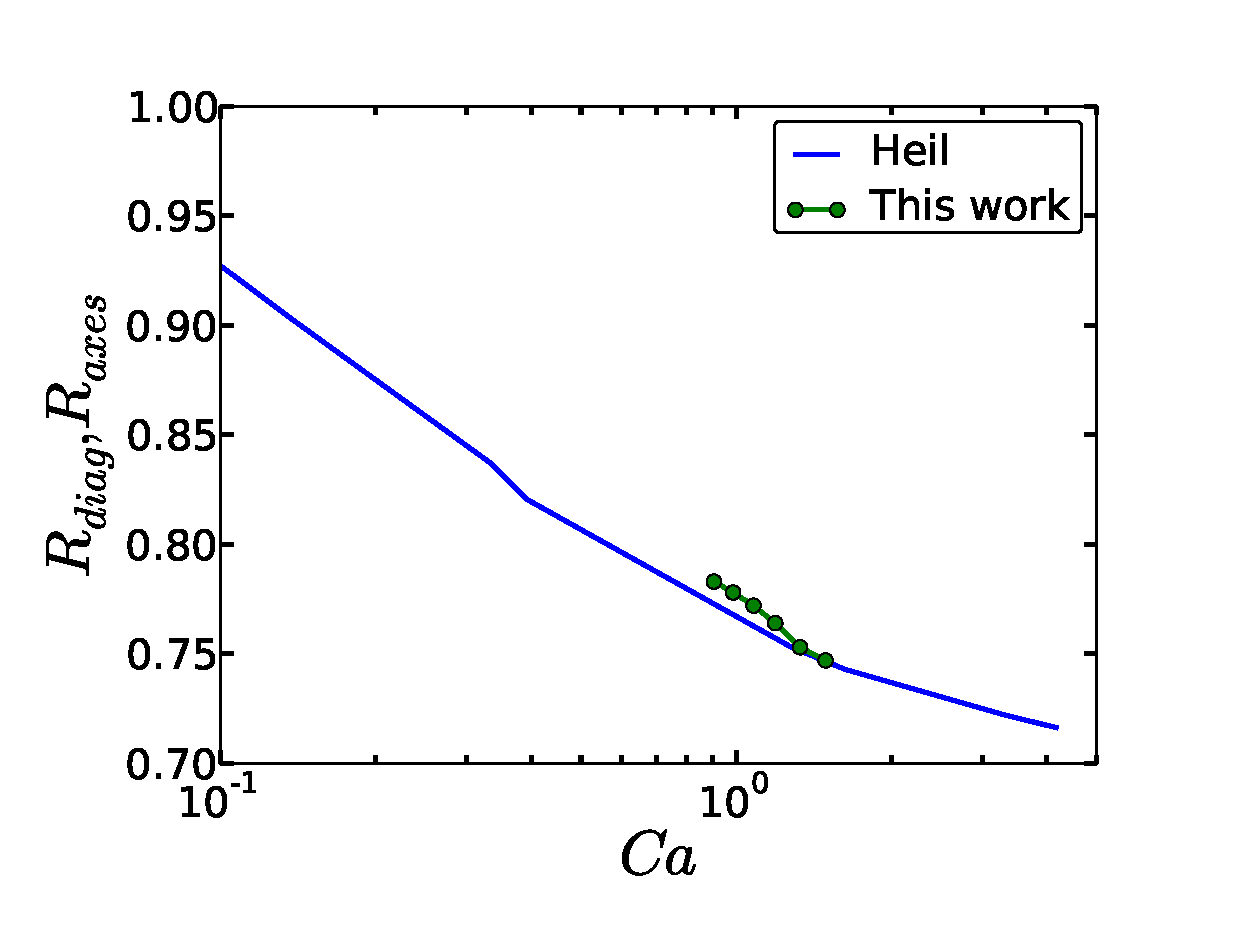
\includegraphics[width=0.97\textwidth]{Figures/capillaries_comparison_train.eps}
\caption{The comparison for the film thickness between \citet{heil-threedim} data and bubble train
simulations. Though, one can see that the decrease of the distance between bubbles causes the
increase in the associated capillary number, however, the correlation dependance between film
thickness and capillary number stays the same. This can help for simulations to reduce the
numerical domain. \label{fig:capillaries:train}}
\end{figure}

\section{Conclusion}
The present work conducts the binary-liquid simulations with the lattice Boltzman method. The
method is a continuous interface method. Along with similarity of results with already published
results of \citet{heil-threedim} and \citet{wang-non-circular}, the differencies were found,
especially in the velocity pattern. Results evedince that the lattice Boltzmann binary liquids
simulations can be used for simulation of gas bubbles in the microchannel. 

\appendix
\section{Symmetric boundary conditions}
\label{append:sym}
For the memory save we performed the simulation of the quarter of the channel while using the
antisymmetric boundary conditions. In the macroscopic variables the mirror boundary conditions
require to have the same scalar fields, but for velocity only tangential velocities are the same
but perpendicular have the opposite directions. This implies the following in terms of the
macroscopic variables:
\begin{equation}
\rho_B = \rho_F, \quad \phi_B = \phi_F \quad U_{B\tau}=U_{F\tau}, U_{B n}=U_{F n}, 
\end{equation}
 where $B$ and $F$ stand for the boundary and the nearest fluid node, respectively. 

In terms of the lattice Boltzmann populations this conditions require the same set of the
populations for the boundary node as for the fluid node. However, the set is mirrored against the
plane of the boundary. This case allows to conserve scalar fields, to have the same tangential
velocities and to have opposite normal velocities. The grid was chosen as 52x52x1500, which is the
effective calculated domain as 100x100x1500 grid nodes. 

\section{Scaling procedure}
\label{append:scaling}
For scaling purposes one need to obtain setup a body force as $\frac{\mathrm{d}P}{\mathrm{d}x}$. If
one obtained a certain velocity of the bubble with the associated gradient then another gradient
can be obtained through the porpotionality condition as:
\begin{equation}
\frac{\mathrm{d}P}{\mathrm{d}x}=\frac{8}{N_y^2} \gamma Ca,
\end{equation}
or in other words th functionality can be extended as:
\begin{equation}
\dfrac{\dfrac{\mathrm{d}P_1}{\mathrm{d}x}}{\dfrac{\mathrm{d}P_2}{\mathrm{d}x}}=\frac{Ca_1}{Ca_2}
\frac{N_{
y2}^2 }{N_{y1}^2}
\end{equation}


\bibliographystyle{unsrtnat}
\bibliography{paper}
\end{document}


